%Copyright 2021 Jean-Michel Bruel
%This program is free template, under the terms of the attached License of this repo.
%Based on https://github.com/jpeisenbarth/SRS-Tex
%Itself based on the code of Yiannis Lazarides
%http://tex.stackexchange.com/questions/42602/software-requirements-specification-with-latex
%http://tex.stackexchange.com/users/963/yiannis-lazarides
%Also based on the template of Karl E. Wiegers
%http://www.se.rit.edu/~emad/teaching/slides/srs_template_sep14.pdf
%http://karlwiegers.com
\documentclass{scrreprt}
\usepackage{method}		% Specific command from Handbook
\usepackage{minitoc}	% For table of content in chapters
\usepackage{listings}
\usepackage{underscore}
\usepackage{booktabs}
\usepackage{tabularx}
\usepackage{xltabular}
\usepackage[a4paper,margin=25mm]{geometry}
\usepackage{microtype}
\setlength{\emergencystretch}{2em}
\usepackage{float}
\usepackage{needspace}
\usepackage{pdflscape}
\usepackage{graphicx}
\usepackage[numbers]{natbib}
\usepackage[bookmarks=true]{hyperref}
\usepackage[utf8]{inputenc}
\usepackage[english]{babel}
\hypersetup{
    hypertexnames=false,
    bookmarks=false,    % show bookmarks bar?
    pdftitle={Software Requirement Specification},    % title
    pdfauthor={Group 7},                     % author
    pdfsubject={Natural Control requirements draft},                        % subject of the document
    pdfkeywords={accessibility, voice, agent supervision, requirements}, % list of keywords
    colorlinks=true,       % false: boxed links; true: colored links
    linkcolor=blue,       % color of internal links
    citecolor=black,       % color of links to bibliography
    filecolor=black,        % color of file links
    urlcolor=purple,        % color of external links
    linktoc=page            % only page is linked
}%
\def\myversion{0.1 }
\date{}
%\title{%

%}
\usepackage{hyperref}
\newcommand*{\nsection}[1]{
    \section*{#1}
    \addcontentsline{toc}{section}{#1}
}
% Numbering
\usepackage{amsthm}
\usepackage{xassoccnt}
%\newtheorem{req}{Requirement}[section]
\newtheorem{req}{Requirement}
\theoremstyle{definition}
\newtheorem{constraint}{Constraint}
\newtheorem{goal}{Goal}
\DeclareCoupledCountersGroup{theorems}
\DeclareCoupledCounters[name=theorems]{req,constraint,goal}
\setcounter{goal}{0}
% Comments
\newcommand{\mynote}[3][black]{\textcolor{#1}{\fbox{\bfseries\sffamily\scriptsize{#2}}
{\small\textsf{\emph{#3}}}}}
\newcommand{\comment}[1]{\mynote[red]{Comment:}{#1}}
%\newcommand{\comment}[1]{}
\newcommand{\notEmpty}{\comment{This chapter should not be empty!}}

\begin{document}

\begin{titlepage}
\begin{flushright}
    \rule{\linewidth}{2pt}\vskip1cm
    \begin{bfseries}
        \Huge{SOFTWARE REQUIREMENTS\\ SPECIFICATION}\\
        \vspace{1.1cm}
        for\\
        \vspace{1.1cm}
        Natural Control\\
        \vspace{1.1cm}
        \LARGE{Version \myversion (draft)}\\
        \vspace{1.1cm}
        Prepared by Group 7\\
        \Large{Lucas DeBoer, Kevin Kim, Aaron Loh, Curtis Vos}\\
        \vspace{1.1cm}
        Group 7, SFWRENG 4G06, McMaster University\\
        \vspace{1.1cm}
        \today\\
    \end{bfseries}
\end{flushright}
\end{titlepage}

\chapter*{Revision History}

\begin{center}
    \begin{tabular}{|c|c|c|c|}
        \hline
	    Name        & Date          & Reason For Changes & Version\\
        \hline
        \hline
	    Aaron Loh & 2026-10-14    & First draft from team planning decisions & 0.1\\
        Aaron Loh & 2026-10-17 & Supervision rules and layout review & 0.1\\
        \hline
    \end{tabular}
\end{center}

This document follows the requirements documentation structure presented in the \href{ https://link.springer.com/content/pdf/10.1007/978-3-031-06739-6.pdf}{Handbook of requirements and business analysis}, by Bertrand Meyer, with the changes listed in the first chapter.

\comment{Working draft. Red comment boxes mark decisions and writing the team still owns. Goals G1 to G5 refer to the Problem Statement goals.}

\dominitoc% Initialization
\tableofcontents
\adjustmtc

\chapter*{Changes from the Meyer template}
\addcontentsline{toc}{chapter}{Changes from the Meyer template}

\begin{itemize}
    \item Glossary moved to the front, so every term is defined before first use.
    \item Added G.8 User profiles, to describe distinct user groups and their needs.
    \item Added E.7 Standards and legal/regulatory factors, plus environment requirements.
    \item S.2 split into one subsection per component, with safety requirements ported from the Hazard Analysis.
    \item Added S.4 Normal operation, S.5 Undesired event handling, and S.9 Formalization (task state machine).
    \item Added requirement dependencies (traceability) and References.
\end{itemize}

\chapter*{Glossary}
\addcontentsline{toc}{chapter}{Glossary}

Project terms:

\begin{itemize}
    \item User: the person who owns the connected accounts and gives commands. Other voices in the room are not users.
    \item Setup helper: a person who completes the initial assisted setup for the user.
    \item Session: the period during which the user is talking with the system, started and ended with the client's start control or a keyboard shortcut, or ended by disconnection. A session can contain several tasks.
    \item Task: one job the user asks for. It may pause before it is completed, cancelled, or failed.
    \item Consequential action: a write to user or account data, a submission, an external message, or a commitment such as accepting terms or granting access. Navigation and temporary preparation do not need approval unless they cause one of these effects. FR24 defines one exception for rejecting non-essential cookies.
    \item Approval: the user's explicit consent to one consequential action, or to a listed batch of similar actions, with their specific details; used once and void if any detail changes.
    \item Barge-in: the user speaking while the system is speaking; it stops the speech only.
    \item Stop request: an explicit ``stop working'' command or stop key. It pauses work and preserves the task. Cancellation ends the task.
    \item Pause acknowledged: the system received the stop request. Pause confirmed: no new task actions can start. Any earlier operation that is still pending is reported separately.
    \item Verified outcome: a result supported by a matching tool response, account record, or website confirmation. Unknown outcome: an action whose result cannot be determined.
\end{itemize}

Technical terms: LiveKit, Hermes, Browser Use, MCP (Model Context Protocol), OAuth, VoiceOver, STT (speech-to-text), TTS (text-to-speech), LLM (large language model), POC (proof of concept).

\comment{Add a one-line definition and an online reference link for each technical term, as AlgoCatan did.}

\chapter*{Goals}
\addcontentsline{toc}{chapter}{Goals book}
\minitoc

\nsection{G.1 Context and overall objective}

Many websites and applications communicate information, choices, and state changes visually. Blind users can face barriers completing multi-step digital tasks and knowing whether those tasks succeeded. Natural Control is a voice interface that lets a blind user delegate tasks in a web browser and in Gmail and Google Calendar to an AI agent, while staying informed and in control.

\nsection{G.2 Current situation}

Today, blind users complete these tasks with screen readers such as VoiceOver, navigating each interface element by element, or with help from a sighted person. Existing AI computer-use agents assume the user can watch the screen to monitor and correct them.

In an interview with a former CNIB Deafblind Community Services (DBCS) staff member on October 17, 2026, the participant observed that screen readers are hard to learn for older, newly diagnosed users and often read irrelevant content, and that everyday tasks such as booking appointments often need a friend's help.

\comment{Add findings from blind participants once sessions start.}

\nsection{G.3 Expected benefits}

\begin{itemize}
    \item Delegate, don't navigate: the user simply states an outcome (``reply to Alex'') instead of visually navigating the interface step by step. (G1)
    \item Control without sight: the user can understand, approve, correct, and stop the agent without seeing the screen. (G2, G4)
    \item Trustworthy results: results are checked against the real account or page before being reported, so the user does not need sighted help to confirm what happened. (G3)
\end{itemize}

\comment{Support each benefit with evidence (interview findings, prior research).}

\nsection{G.4 Functionality overview}

The user starts a session from the web client and speaks a task. The system clarifies missing details, carries out read-only steps on its own, asks for approval before every consequential action, reports progress and verified results by voice, and accepts corrections and stop requests at any time. A task history records what happened.

\nsection{G.5 High-level usage scenarios}

\begin{itemize}
    \item Reply to an email.
    \item Add an event found on a webpage to the calendar.
    \item Compare information on an unfamiliar website.
    \item Correct or stop a running task.
    \item Reconnect after a dropped connection without duplicating an action.
\end{itemize}

\comment{Draw a use case or activity diagram for these scenarios.}

\nsection{G.6 Limitations and exclusions}

\begin{itemize}
    \item Native Mac application control and general local-file tasks.
    \item Platforms other than Mac with Chrome; languages other than English.
    \item Phone calling and saved workflows (stretch goals).
    \item Background continuation: tasks always pause when the user disconnects; continuing unattended is a possible extension.
    \item Fully local model inference; the system uses cloud AI and speech providers.
    \item Users who cannot hear spoken output, including many deafblind users. Braille output through VoiceOver is a possible extension.
\end{itemize}

\nsection{G.7 Stakeholders and requirements sources}

\begin{itemize}
    \item Primary: blind and visually impaired people who want to complete digital tasks without visual feedback. Initial evaluation: blind Mac users with screen-reader experience.
    \item Secondary: other people who want nonvisual interaction.
    \item Tertiary: website and application developers who affect the system's operational limits.
    \item Setup helper: a person who completes the assisted setup.
    \item Requirements sources: the Problem Statement, Development Plan, and Hazard Analysis; TA and instructor guidance; prior research (WebAIM survey, Morae); an interview with a former CNIB Deafblind Community Services (DBCS) staff member on October 17, 2026; and planned participant sessions.
    \item Intervenors: support workers who may help deafblind users with setup and recovery.
\end{itemize}

\nsection{G.8 User profiles}

\begin{itemize}
    \item Experienced screen-reader user: fluent with VoiceOver or JAWS and keyboard navigation; wants speed on multi-step tasks and keeps their screen reader for everything else. Primary evaluation group.
    \item Less experienced or recently blind user: often older, with acquired vision loss, limited screen-reader skill, and possibly an older device; benefits most from delegation and clear spoken confirmation.
    \item Sighted user wanting nonvisual interaction: can see the screen but prefers or needs voice (busy hands, away from the screen); can verify visually, so has lower risk.
    \item Setup helper: comfortable with computers; connects accounts and grants permissions once, then is not needed for daily use.
\end{itemize}

\comment{Validate these profiles with blind participants; drop or adjust any that do not hold up.}

\chapter*{Environment}
\addcontentsline{toc}{chapter}{Environment book}
\minitoc

\nsection{E.1 Glossary}

See the Glossary at the front of this document.

\nsection{E.2 Components}

\begin{itemize}
    \item Websites the user asks about (unmodified, not under our control).
    \item Google services: Gmail and Google Calendar APIs.
    \item Composio: hosted service that stores OAuth tokens and runs Gmail and Calendar tool calls. Its ``Don't store data'' setting is turned on so tool inputs and outputs are not logged.
    \item LiveKit (real-time audio and speech pipeline).
    \item AI model and speech providers.
    \item The Hermes agent and Browser Use (reused open-source components).
    \item VoiceOver and the Mac's microphone and speakers.
    \item Network access.
\end{itemize}

\nsection{E.3 Constraints}

\begin{itemize}
    \item Mac with Chrome, English, as decided in the Development Plan.
    \item Team budget ceiling of \$500 CAD.
    \item Course schedule: POC demonstration November 23 to December 3; final demonstration and EXPO in April.
    \item Gmail and Calendar access uses restricted Google OAuth permissions. An app in Testing status is capped at 100 registered test users, and its issued refresh tokens expire after 7 days, requiring re-authorization until the app is verified or published \citep{GoogleOAuthLimits}.
    \item Provider terms of use and data retention policies apply to anything sent to them.
    \item Passwords and payment details are entered through a private page or the user's own device. One-time authentication codes may be spoken. Spoken codes pass through the configured speech and conversation services. Provider handling must be checked before claiming stronger privacy guarantees.
\end{itemize}

\nsection{E.4 Assumptions}

\begin{itemize}
    \item A setup helper completed setup correctly (accounts connected, permissions granted).
    \item Only the user gives commands; other voices are noise.
    \item Connected accounts belong to the user; development and evaluation use test accounts.
    \item The user can hear spoken output (see G.6).
\end{itemize}

Speech recognition, the AI model, websites, and external services are not assumed to work correctly; their failures are covered by the Hazard Analysis and S.5.

\nsection{E.5 Effects}

\begin{itemize}
    \item Emails are searched, read, drafted, sent, replied to, archived, labelled, or deleted.
    \item Calendar events are read, created, updated, or deleted.
    \item Website forms may be filled and submitted, subject to approval.
    \item Data is sent to AI and speech providers.
\end{itemize}

\nsection{E.6 Invariants}

\begin{itemize}
    \item Writes and consequential commitments require approval of their exact details. FR24 defines the narrow exception for rejecting non-essential cookies.
    \item The user's existing accessibility tools (VoiceOver, keyboard navigation) keep working while the system runs.
    \item Credentials are never written to source control, logs, or task history.
\end{itemize}

\nsection{E.7 Standards and legal/regulatory factors}

\begin{itemize}
    \item WCAG 2.2 Level AA: accessibility standard for the web client, adopted voluntarily \citep{WCAG22}.
    \item AODA (Accessibility for Ontarians with Disabilities Act): Ontario accessibility law referencing WCAG; its compliance obligations are not required as they apply to organizations with Ontario employees (20+ for reporting, 50+ for website compliance), but it is a relevant reference for our team \citep{AODAFactSheet}.
    \item Google API Services User Data Policy: binds the project as a condition of using Gmail and Calendar APIs regardless of organizational status; limits how that data may be used and stored \citep{GoogleAPIDataPolicy}.
    \item Open-source licenses: our code uses MIT licensing; reused components keep their own licenses and notices.
    \item Coding standards: PEP 8 for Python; strict TypeScript with a shared linter for the client.
\end{itemize}

\subsection*{Environment requirements}
\addcontentsline{toc}{subsection}{Environment requirements}

\begin{itemize}
    \item NFR.E.1: The system shall run on macOS with Google Chrome.
    \item NFR.E.2: The web client shall meet WCAG 2.2 Level AA.
    \item NFR.E.3: The system shall use Gmail and Calendar data only to perform the user's requested tasks, consistent with the Google API Services User Data Policy.
    \item NFR.E.4: Python code shall pass the team's PEP 8 linter checks; TypeScript code shall pass strict type checks and the shared linter.
\end{itemize}

\chapter*{System}
\addcontentsline{toc}{chapter}{System book}
\minitoc

\Needspace{8\baselineskip}
\nsection{S.1 Components}

The proposed system has eight components. These match the Hazard Analysis. Figure~\ref{fig:components} shows their connections and external services. Team-owned components are planned work. The POC must test the integration boundaries.



\begin{itemize}
    \item \textbf{Accessible client:} the web interface for sessions and task history. It provides keyboard controls and works alongside VoiceOver.
    \item \textbf{Voice interface:} uses LiveKit for audio and conversational turn handling. Our integration passes requests and corrections to the task manager. It speaks relevant questions and results.
    \item \textbf{Task manager:} starts tasks and tracks their state. It handles corrections, pauses, cancellation, and resumption (S.9).
    \item \textbf{AI agent:} Hermes plans tasks and proposes tool calls. Each call must pass through the action gate.
    \item \textbf{Action gate:} checks every proposed action. It requests approval for writes and consequential commitments. Approval details come from the proposed call. The gate also blocks new task actions while work is paused.
    \item \textbf{Outcome verification:} checks evidence for each consequential action. Evidence may come from its tool response or a targeted account or page check. The result is recorded as verified, partial, failed, or unknown.
    \item \textbf{Action tools and integrations:} Browser Use handles websites. Gmail and Google Calendar tools use the Composio SDK. The proposed integration places approval checks before execution and outcome checks afterward. The POC must verify that all action paths pass through these checks. Credential handling also needs verification.
    \item \textbf{Task history layer:} records task state and action outcomes. It also records approvals and action IDs. These records support accessible review and recovery after disconnection.
\end{itemize}

\begin{landscape}
\begin{figure}[p]
\centering
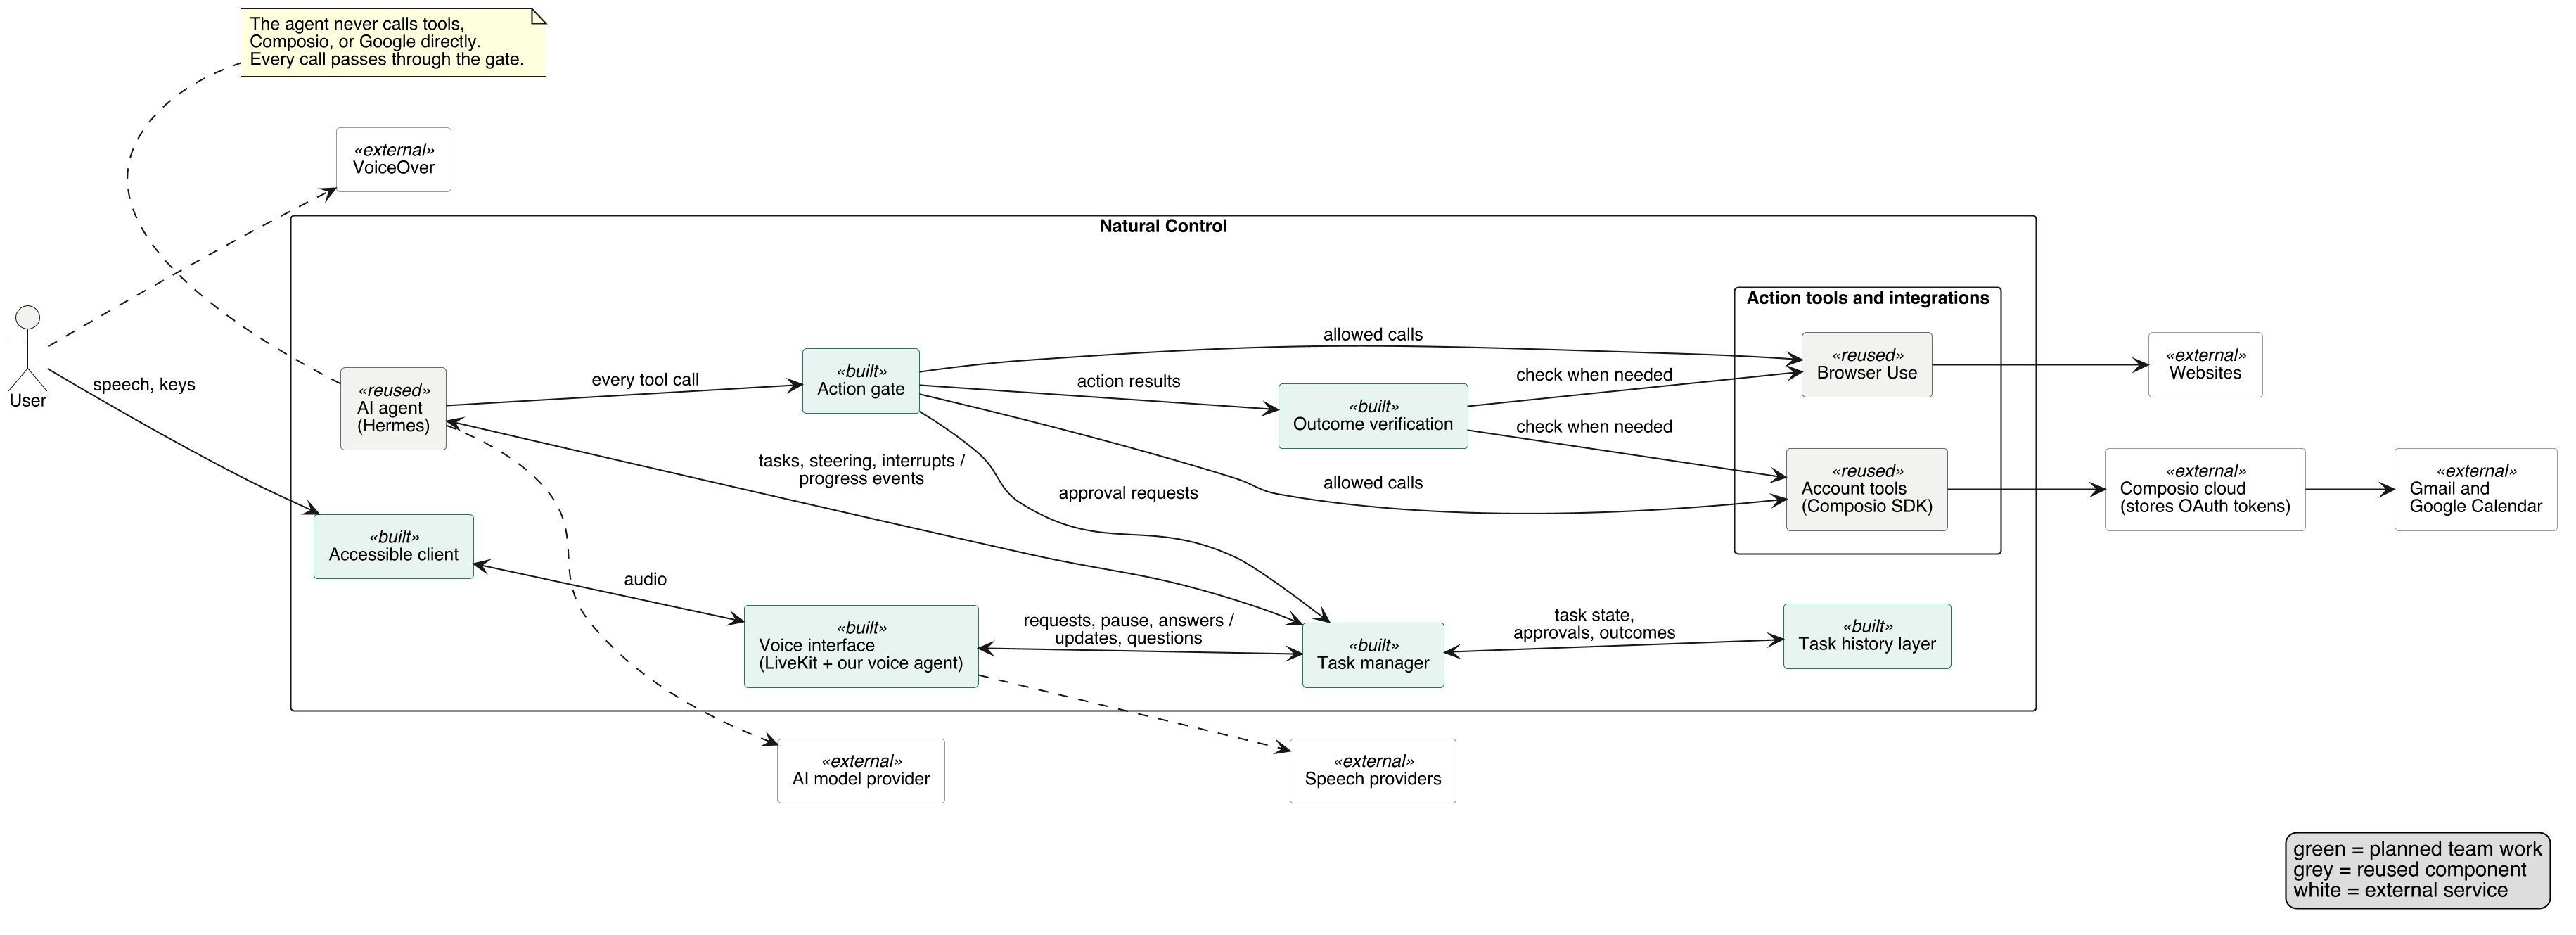
\includegraphics[width=\linewidth,height=.65\paperwidth,keepaspectratio]{figures/component-diagram.png}
\caption{Component diagram. Green components are planned team work. Grey components are reused. White boxes are external services.}
\label{fig:components}
\end{figure}
\end{landscape}

\Needspace{8\baselineskip}
\nsection{S.2 Functionality}

Requirements are grouped by their responsible component (S.1). Each has a rationale and trace links. G1 to G5 refer to project goals. FR.Sa and NFR.Sa refer to safety requirements. The task manager and action gate constrain the AI agent. Outcome verification checks its results.

\Needspace{12\baselineskip}
\subsection*{S.2.1 Voice interface}
\addcontentsline{toc}{subsection}{S.2.1 Voice interface}

\begingroup
\small
\begin{xltabular}{\textwidth}{>{\raggedright\arraybackslash}p{1cm}>{\hsize=1.3\hsize\raggedright\arraybackslash}X>{\hsize=.7\hsize\raggedright\arraybackslash}X>{\raggedright\arraybackslash}p{2cm}}
\caption{Voice interface requirements}\label{tab:fr1}\\
\toprule
\textbf{ID} & \textbf{Requirement} & \textbf{Rationale} & \textbf{Traces to}\\
\midrule
\endfirsthead
\toprule
\textbf{ID} & \textbf{Requirement} & \textbf{Rationale} & \textbf{Traces to}\\
\midrule
\endhead
\bottomrule
\endfoot
FR1 & The system shall accept spoken input during a session. It shall support pauses within a thought through the selected voice framework's turn handling. & Voice is the main input for everyday use. Turn timing needs POC and user evaluation. & G1\\\addlinespace[4pt]
FR2 & The user shall be able to interrupt spoken output. This shall not restart the task or pause its execution by itself. A correction or explicit work-stop request shall follow its own handling. & Users need to cut off long speech without losing work. & G2\\\addlinespace[4pt]
FR3 & An explicit ``stop working'' command or the stop key shall pause the task (FR8). A bare ``stop'' shall stop speech and pause work. The system shall clarify what the user wants next. An explicit request to cancel or abandon the task shall end it. & Speech interruption, work pause, and cancellation have different effects. The key provides a backup when voice fails. & G2; FR.Sa.1, FR.Sa.4\\\addlinespace[4pt]
FR16 & The system shall let the user correct part of a read-back (for example, one sentence or one detail) by voice without restarting the request. & Interview: fixing a read-back usually means starting over. Correcting speech input is slow for blind users [Azenkot and Lee 2013]. & G4\\\addlinespace[4pt]
FR18 & Spoken updates and summaries shall include only information relevant to the current task, with more detail available on request. & Interview and WebAIM survey: screen readers read too much irrelevant content. & G2\\\addlinespace[4pt]
\end{xltabular}
\endgroup

\Needspace{12\baselineskip}
\subsection*{S.2.2 Task manager}
\addcontentsline{toc}{subsection}{S.2.2 Task manager}

\begingroup
\small
\begin{xltabular}{\textwidth}{>{\raggedright\arraybackslash}p{1cm}>{\hsize=1.3\hsize\raggedright\arraybackslash}X>{\hsize=.7\hsize\raggedright\arraybackslash}X>{\raggedright\arraybackslash}p{2cm}}
\caption{Task manager requirements}\label{tab:fr2}\\
\toprule
\textbf{ID} & \textbf{Requirement} & \textbf{Rationale} & \textbf{Traces to}\\
\midrule
\endfirsthead
\toprule
\textbf{ID} & \textbf{Requirement} & \textbf{Rationale} & \textbf{Traces to}\\
\midrule
\endhead
\bottomrule
\endfoot
FR4 & The system shall ask when required details are missing or ambiguous. It shall recheck relevant information before continuing. & Guessing risks acting on the wrong item. & G3; FR.Sa.9\\\addlinespace[4pt]
FR5 & The system shall report meaningful progress and blockers. It shall answer requests for current status. Routine updates shall follow the task and conversation rather than a fixed interval. Pending questions and approvals shall not expire while the user remains connected. & Users need awareness without constant narration. Silence is not approval. & G2; NFR.Sa.3\\\addlinespace[4pt]
FR6 & The system shall accept corrections during a task without requiring a restart. & Restarting a long task by voice is costly. & G4\\\addlinespace[4pt]
FR7 & Disconnection shall pause the task as in FR8. On reconnection the system shall report its state and reconcile uncertain outcomes. It shall wait for a clear request to resume work. & Reconnecting the voice session does not authorize more actions. & G2, G4; FR.Sa.7\\\addlinespace[4pt]
FR8 & A stop request shall block new task actions and preserve task context. The system shall stop or suspend ongoing work where safe and supported. An operation already submitted may settle if it cannot be stopped safely. The system shall distinguish acknowledgment from confirmed pause. It shall report completed work and unfinished work. It shall also report any outcome still unknown. Checks during a pause shall only reconcile earlier actions. Work shall resume only on a clear user request. & Pausing does not undo a submitted action. The user needs an accurate account of what remains. & G2, G4; FR.Sa.5\\\addlinespace[4pt]
FR19 & A new request during an active task shall be treated as a correction when that is clear. Otherwise the system shall ask whether to queue it or replace the current task. Replacement shall end the earlier task before the new one starts. & One active task keeps spoken progress easy to follow (S.9, P6). & G2\\\addlinespace[4pt]
FR20 & When the user moves to another request the system shall withdraw pending questions and approvals. It shall state that the pending action was not executed. It shall distinguish this from earlier completed work. The new request shall follow FR19. & An abandoned approval must not be used later. & G2, G3; FR.Sa.15\\\addlinespace[4pt]
FR21 & At session start the system shall announce paused tasks and their last known state. The user may resume or cancel. Before resuming the system shall check relevant state and reconcile earlier actions. Pending approvals shall be requested again. Reconnection alone shall not resume work. & Recovery must preserve context without repeating actions. & G2, G4; FR.Sa.8\\\addlinespace[4pt]
\end{xltabular}
\endgroup

\Needspace{12\baselineskip}
\subsection*{S.2.3 Action gate}
\addcontentsline{toc}{subsection}{S.2.3 Action gate}

\begingroup
\small
\begin{xltabular}{\textwidth}{>{\raggedright\arraybackslash}p{1cm}>{\hsize=1.3\hsize\raggedright\arraybackslash}X>{\hsize=.7\hsize\raggedright\arraybackslash}X>{\raggedright\arraybackslash}p{2cm}}
\caption{Action gate requirements}\label{tab:fr3}\\
\toprule
\textbf{ID} & \textbf{Requirement} & \textbf{Rationale} & \textbf{Traces to}\\
\midrule
\endfirsthead
\toprule
\textbf{ID} & \textbf{Requirement} & \textbf{Rationale} & \textbf{Traces to}\\
\midrule
\endhead
\bottomrule
\endfoot
FR9 & Writes and consequential commitments shall require approval of their exact details. These include sending, saving, deleting, submitting, granting access, and accepting terms. Approval shall be an explicit affirmative answer to the pending approval question. Silence is not approval. Changed details require new approval. FR24 defines the cookie-rejection exception. & Users retain control over changes and commitments. Approval checks use the proposed tool call (ADR 0001). & G2, G3; FR.Sa.3, FR.Sa.13, FR.Sa.14\\\addlinespace[4pt]
FR10 & Reading, navigation, and temporary preparation shall proceed without approval when they cause no consequential effect. Autosaved drafts are writes. A click that submits data is consequential. Unknown effects shall require approval. A failed read-only lookup may be retried once before it is reported as a blocker. & Classify the effect of an action rather than the name of its tool. & G1, G2; FR.Sa.13\\\addlinespace[4pt]
FR11 & Each approved action shall have a unique ID. A completed action shall not be repeated as a retry. Before retrying an uncertain action the system shall check its outcome. If it remains unknown the system shall ask the user. A new attempt requires fresh approval. & An uncertain result must not cause a duplicate write. & G3; FR.Sa.6, FR.Sa.18\\\addlinespace[4pt]
FR13 & The system shall treat webpage and email content as data, never as instructions. & Websites and emails can contain text written to manipulate agents. & FR.Sa.16\\\addlinespace[4pt]
\end{xltabular}
\endgroup

\paragraph{Approval details.} Similar actions may share one approval. The read-back shall state the number of actions, the intended changes, and a concise description identifying the affected items. Full item details shall be available on request. The approved batch shall retain each item's identity and exact details. Each item may run once. Partial failures shall be reported per item. A pause shall block remaining items and withdraw their unused approvals.

For email the read-back shall name the recipients and subject. It shall read the body in full up to SHORT\_MESSAGE\_LENGTH. For longer messages it shall give a summary and offer the full text. The user may request a sentence-by-sentence read-back. A reduced-prompt permission mode is deferred.

\Needspace{12\baselineskip}
\subsection*{S.2.4 Outcome verification}
\addcontentsline{toc}{subsection}{S.2.4 Outcome verification}

\begingroup
\small
\begin{xltabular}{\textwidth}{>{\raggedright\arraybackslash}p{1cm}>{\hsize=1.3\hsize\raggedright\arraybackslash}X>{\hsize=.7\hsize\raggedright\arraybackslash}X>{\raggedright\arraybackslash}p{2cm}}
\caption{Outcome verification requirements}\label{tab:fr4}\\
\toprule
\textbf{ID} & \textbf{Requirement} & \textbf{Rationale} & \textbf{Traces to}\\
\midrule
\endfirsthead
\toprule
\textbf{ID} & \textbf{Requirement} & \textbf{Rationale} & \textbf{Traces to}\\
\midrule
\endhead
\bottomrule
\endfoot
FR12 & Each consequential result shall be reported as verified, partial, failed, or unknown. Evidence shall match the intended action and details. It may be a completion response from the connector, a matching account record, or a website confirmation. Another check is required when that evidence is unclear. A queued request shall not be reported as delivered. & The reported result must match the available evidence. A second lookup is not always needed. & G3; FR.Sa.10\\\addlinespace[4pt]
\end{xltabular}
\endgroup

\Needspace{12\baselineskip}
\subsection*{S.2.5 Action tools and integrations}
\addcontentsline{toc}{subsection}{S.2.5 Action tools and integrations}

\begingroup
\small
\begin{xltabular}{\textwidth}{>{\raggedright\arraybackslash}p{1cm}>{\hsize=1.3\hsize\raggedright\arraybackslash}X>{\hsize=.7\hsize\raggedright\arraybackslash}X>{\raggedright\arraybackslash}p{2cm}}
\caption{Action tools and integrations requirements}\label{tab:fr5}\\
\toprule
\textbf{ID} & \textbf{Requirement} & \textbf{Rationale} & \textbf{Traces to}\\
\midrule
\endfirsthead
\toprule
\textbf{ID} & \textbf{Requirement} & \textbf{Rationale} & \textbf{Traces to}\\
\midrule
\endhead
\bottomrule
\endfoot
FR14 & The system shall request only the account permissions it needs, and explain them during setup, including which providers receive which data. & Narrow permissions limit the damage any other failure can do. & G5; FR.Sa.17\\\addlinespace[4pt]
FR17 & The user shall be able to mark topics or accounts as off-limits. The system shall not read or act on them. & The proxy interview raised concerns about sensitive account data. & G2\\\addlinespace[4pt]
FR23 & Website passwords shall be entered through a private setup page and stored encrypted. They shall not be spoken or placed in the conversation. Saved credentials shall be used only for their intended site. The user may speak a one-time authentication code or approve a push on their device. The system shall explain that spoken codes pass through the configured speech and conversation services. A site that requires a device-bound passkey shall use a manual handoff. & Spoken codes can be heard nearby and processed by providers. Private typed code input is a proposed alternative. & G2, G5; FR.Sa.17\\\addlinespace[4pt]
FR24 & The system may automatically choose a clearly identified ``reject non-essential cookies'' or ``necessary only'' option. Any ambiguous consent choice shall require explicit user approval. This is a narrow exception to FR9. Accepting cookies or terms shall require approval. & A limited exception reduces repeated consent prompts. It does not authorize accepting terms. & G2, G3; FR.Sa.13\\\addlinespace[4pt]
\end{xltabular}
\endgroup

\Needspace{12\baselineskip}
\subsection*{S.2.6 Accessible client and task history layer}
\addcontentsline{toc}{subsection}{S.2.6 Accessible client and task history layer}

\begingroup
\small
\begin{xltabular}{\textwidth}{>{\raggedright\arraybackslash}p{1cm}>{\hsize=1.3\hsize\raggedright\arraybackslash}X>{\hsize=.7\hsize\raggedright\arraybackslash}X>{\raggedright\arraybackslash}p{2cm}}
\caption{Accessible client and task history layer requirements}\label{tab:fr6}\\
\toprule
\textbf{ID} & \textbf{Requirement} & \textbf{Rationale} & \textbf{Traces to}\\
\midrule
\endfirsthead
\toprule
\textbf{ID} & \textbf{Requirement} & \textbf{Rationale} & \textbf{Traces to}\\
\midrule
\endhead
\bottomrule
\endfoot
FR15 & The system shall provide accessible task history and spoken summaries from recorded events. The user shall be able to delete that history. & Users need to review what happened without sight. & G2; FR.Sa.2\\\addlinespace[4pt]
FR22 & The client shall provide controls to start and end a voice session. A keyboard shortcut shall also be available. Ending a session shall pause active work as in FR8. & Deliberate activation avoids an always-on microphone. & G2, G5\\\addlinespace[4pt]
\end{xltabular}
\endgroup

\Needspace{12\baselineskip}
\subsection*{S.2.7 Safety requirements}
\addcontentsline{toc}{subsection}{S.2.7 Safety requirements}

The following requirements are SRS revisions based on the Hazard Analysis. Hazard IDs refer to its FMEA rows. The Hazard Analysis remains unchanged. Differences need review by its owner before the documents are submitted.

\paragraph{Functional safety requirements}
\input{FunctionalSafetyRequirements.text}

\paragraph{Non-functional safety requirements}
\input{NonFunctionalSafetyRequirements.text}

\Needspace{12\baselineskip}
\subsection*{S.2.8 Non-functional requirements}
\addcontentsline{toc}{subsection}{S.2.8 Non-functional requirements}

\begingroup
\small
\begin{xltabular}{\textwidth}{>{\raggedright\arraybackslash}p{1cm}>{\hsize=1.3\hsize\raggedright\arraybackslash}X>{\hsize=.7\hsize\raggedright\arraybackslash}X>{\raggedright\arraybackslash}p{2cm}}
\caption{Non-functional requirements}\label{tab:nfr}\\
\toprule
\textbf{ID} & \textbf{Requirement} & \textbf{Rationale} & \textbf{Traces to}\\
\midrule
\endfirsthead
\toprule
\textbf{ID} & \textbf{Requirement} & \textbf{Rationale} & \textbf{Traces to}\\
\midrule
\endhead
\bottomrule
\endfoot
NFR1 & Session controls, work pause, approval, and task history shall work with VoiceOver and the keyboard alone. & Users rely on their existing assistive tools. & G2, G5\\\addlinespace[4pt]
NFR2 & At least TARGET\_COMPLETION of tasks in the declared task suite shall be completed correctly without sighted help. The task suite shall include representative Gmail, Google Calendar, and unfamiliar website tasks. & Measures the main benefit: independent task completion. & G1\\\addlinespace[4pt]
NFR3 & A work-stop request shall be acknowledged within STOP\_ACK\_TIME. Time to block new actions and time to reconcile in-flight work shall be measured separately. & A quick acknowledgment does not prove earlier actions ended. & G2; NFR.Sa.1\\\addlinespace[4pt]
NFR4 & The system shall begin its response within RESPONSE\_TIME after the selected turn detector commits an ordinary request. Premature replies and missed interruptions shall also be evaluated. & Fast replies must not cut off unfinished thoughts. & G2\\\addlinespace[4pt]
NFR5 & The application shall not retain raw microphone audio. It shall exclude credentials and authentication codes from task history, logs, and source control. Setup shall explain provider processing and retention separately. & Application storage rules do not establish provider privacy guarantees. & G5; FR.Sa.17\\\addlinespace[4pt]
\end{xltabular}
\endgroup


\Needspace{16\baselineskip}
Constants below remain provisional. The POC will inform timing choices. Routine speech has no fixed update interval.

\begin{table}[H]
\centering
\small
\caption{Constants}\label{tab:constants}
\begin{tabularx}{\textwidth}{>{\raggedright\arraybackslash}p{4.1cm}>{\raggedright\arraybackslash}X>{\raggedright\arraybackslash}X}
\toprule
\textbf{Constant} & \textbf{Meaning} & \textbf{Value}\\
\midrule
STOP\_ACK\_TIME & Time to audibly acknowledge a work-stop request & TBD after POC (Development Plan provisional: 2 s)\\\addlinespace[4pt]
RESPONSE\_TIME & Time from committed user turn to response start & TBD after POC\\\addlinespace[4pt]
CONNECTION\_NOTICE\_TIME & Time to signal connection loss (NFR.Sa.2) & TBD after POC\\\addlinespace[4pt]
SHORT\_MESSAGE\_LENGTH & Longest email body read in full before approval & TBD after POC\\\addlinespace[4pt]
TARGET\_COMPLETION & Share of tasks completed correctly without sighted help & TBD (Development Plan provisional: 80\%)\\
\bottomrule
\end{tabularx}
\end{table}

\Needspace{8\baselineskip}
\nsection{S.3 Interfaces}

\begin{itemize}
    \item \textbf{User interface:} a web client in Chrome. It provides session controls and task status. The user can pause, resume, or cancel work. Approval details and history are accessible through VoiceOver and the keyboard. Spoken questions can be repeated on request. The system shall explain the keyboard shortcut for stopping work during setup and repeat the shortcut on request. The shortcut shall not conflict with VoiceOver controls.
    \item \textbf{Program interfaces:} LiveKit carries audio and speech events. The Hermes integration carries task requests, corrections, and progress. The task manager controls execution separately from speech. Browser Use and Composio supply action tools. Each tool call passes through the gate.
\end{itemize}

\comment{The voice/client owner must confirm screen layouts and keyboard shortcuts. Private typed code input remains a proposed extension.}

\Needspace{8\baselineskip}
\nsection{S.4 Normal operation}

Figure~\ref{fig:seqnormal} follows one request from start to finish: the user asks to add an event found on a webpage to their calendar.

\begin{enumerate}
    \item The user starts a session from the client (FR22) and speaks the request. The voice interface passes it to the task manager. It records the task and starts the agent in Working. The user hears a short acknowledgment.
    \item The agent reads the page. The action gate lets this read-only call through to Browser Use and screens the returned content for injected instructions (FR10, FR13).
    \item The agent proposes event creation. The gate holds the write and requests approval of its exact details. The task enters AwaitingApproval.
    \item The voice interface reads the details back. The user says ``yes.'' The task manager records approval and releases the call. The task enters Executing (FR9).
    \item The gate submits the call with a unique action ID (FR11). The returned event details confirm creation. Outcome verification checks those details and reports the result (FR12). A separate lookup is used if the response is unclear.
    \item The agent finishes the task (state Done). The task history records each step (FR15), and the user hears the verified result.
\end{enumerate}

\begin{figure}[htbp]
\centering
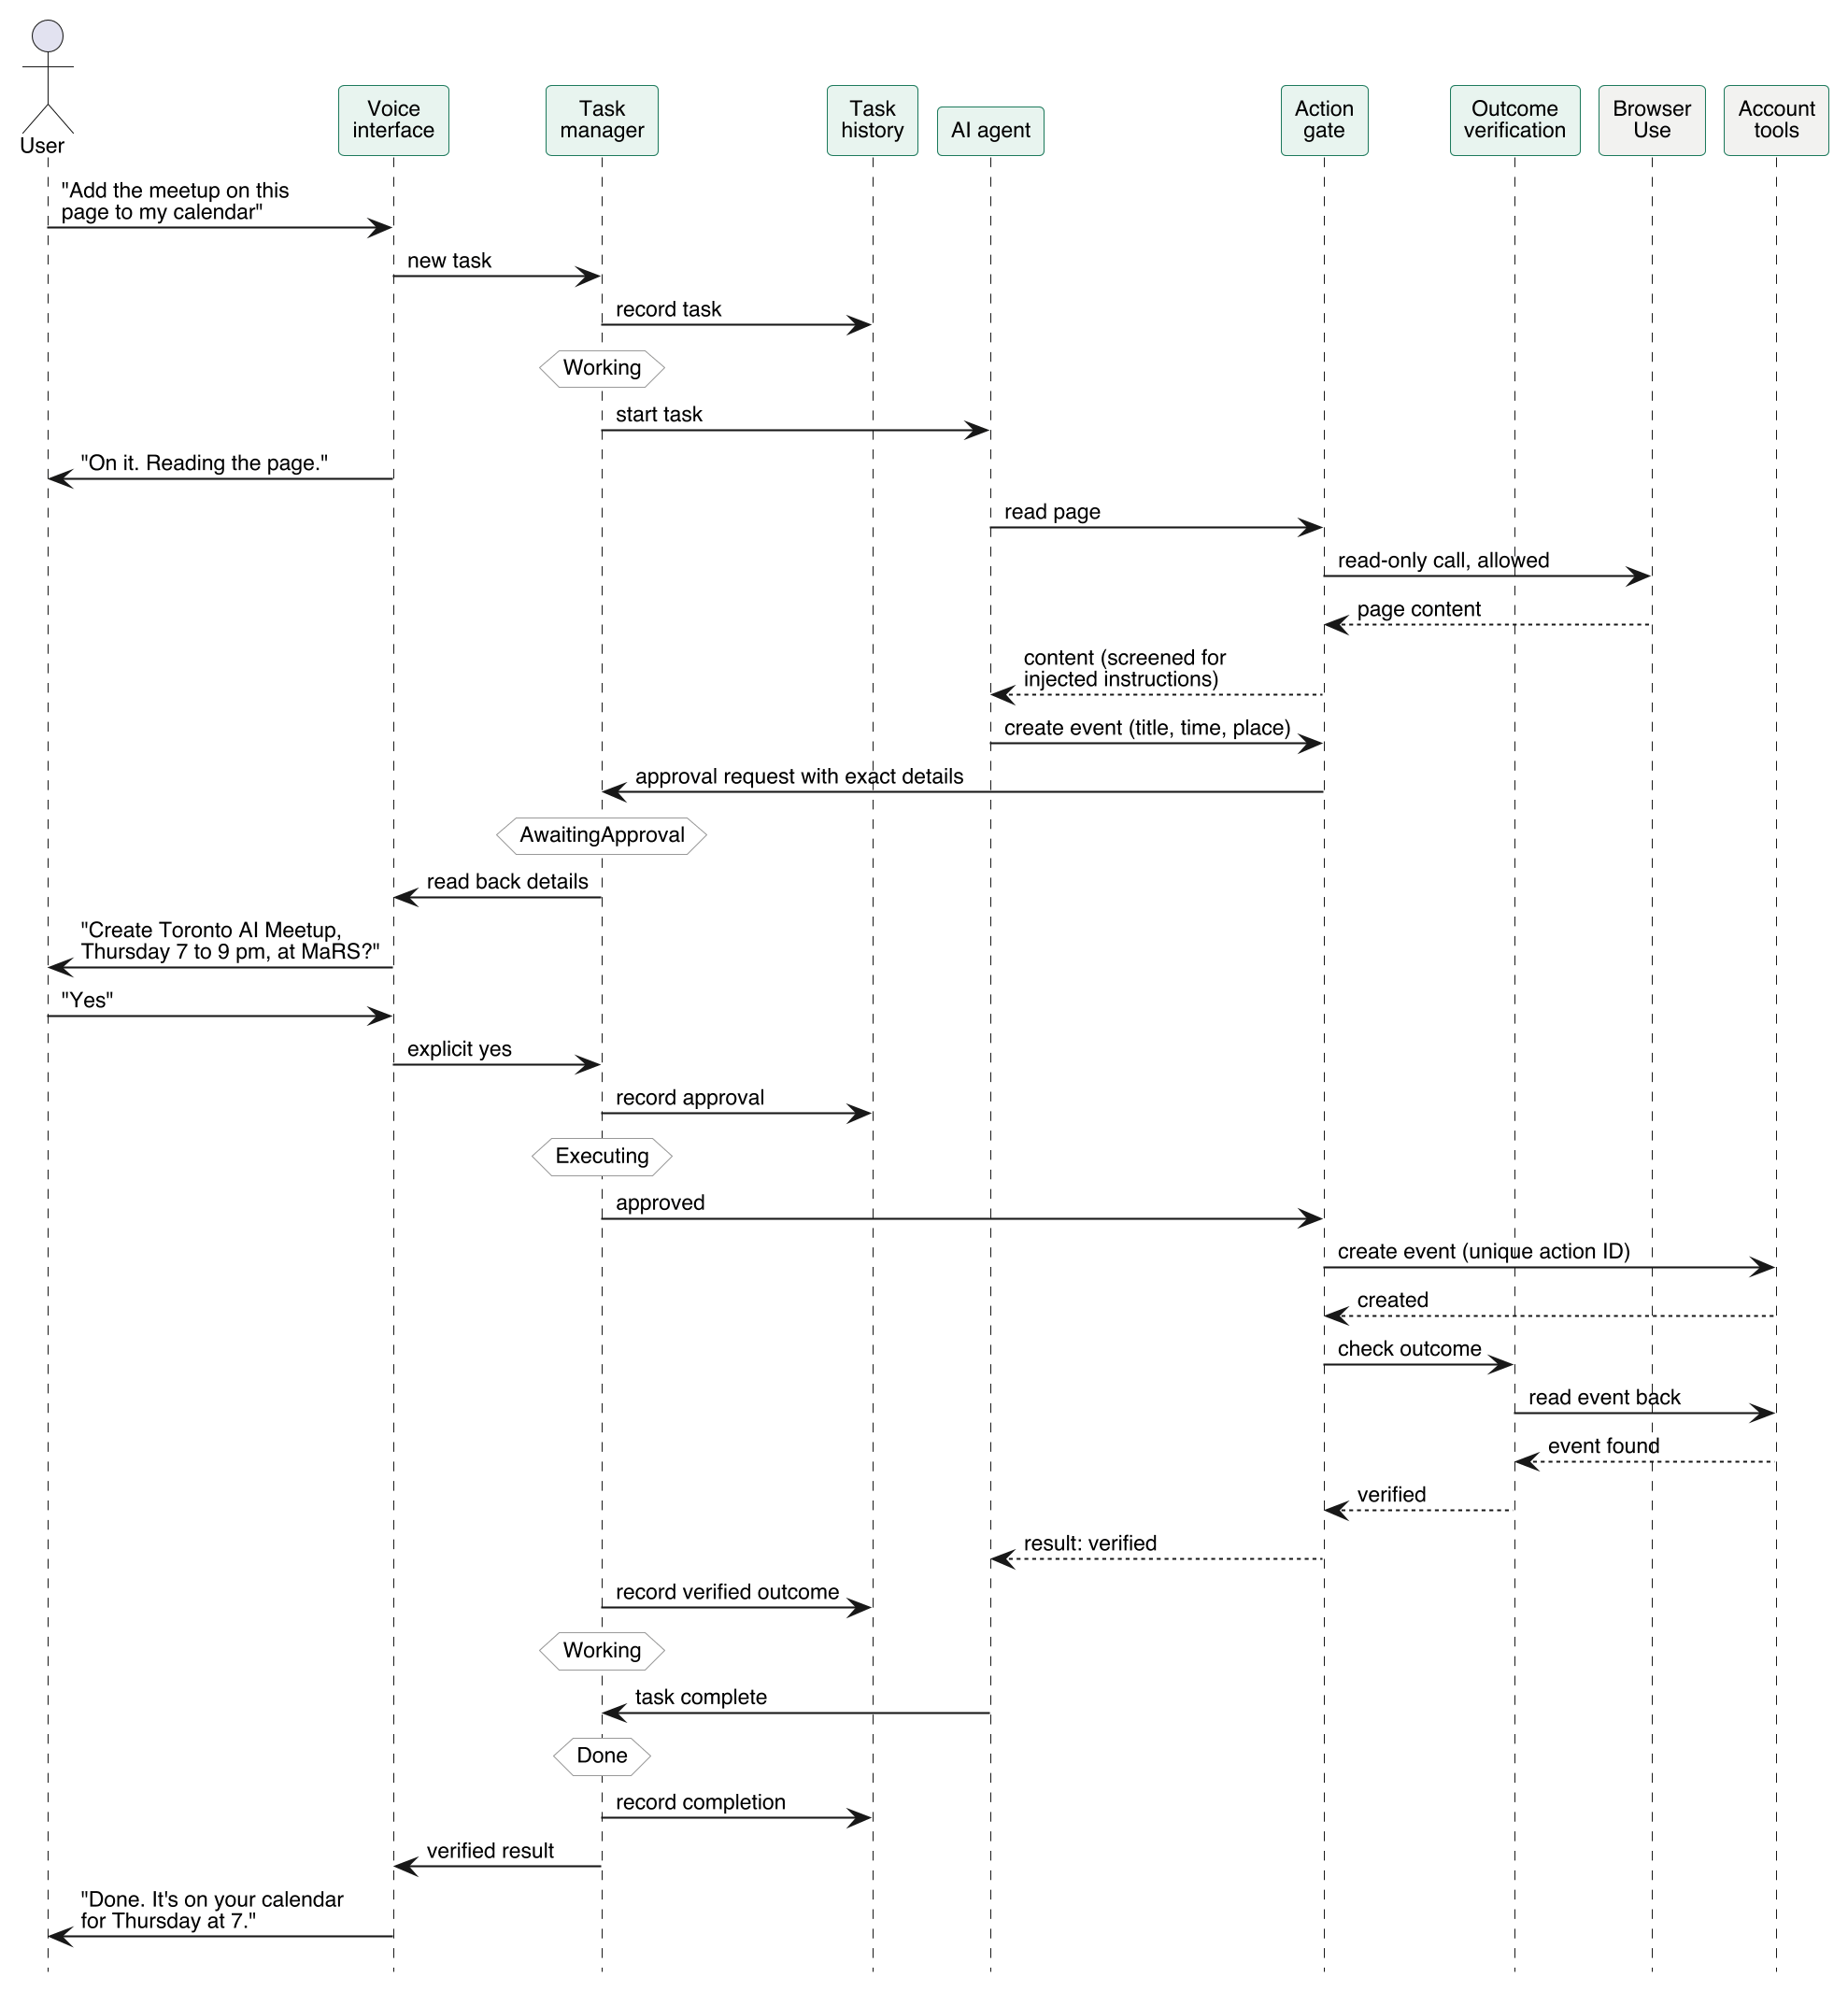
\includegraphics[width=\textwidth,height=.78\textheight,keepaspectratio]{figures/sequence-normal.png}
\caption{Normal operation: adding an event from a webpage to the calendar.}
\label{fig:seqnormal}
\end{figure}

\Needspace{8\baselineskip}
\nsection{S.5 Undesired event handling}

\begin{itemize}
    \item \textbf{Misheard or ambiguous request:} ask for clarification. Read back key details before approval. (H2-a, H4-a)
    \item \textbf{Missed work-stop request:} provide a keyboard backup. Block new task actions once the request is recognized. (H2-b, H3-a)
    \item \textbf{Disconnection:} pause work. Report the state after reconnection and wait for an instruction to resume. (H3-b)
    \item \textbf{Provider failure:} pause work. Explain what completed and what remains unfinished or unknown. (H4-d)
    \item \textbf{Unknown outcome:} check the affected account or page before any retry. Ask the user if the outcome remains unknown. (H7-d)
    \item \textbf{Injected instructions:} treat webpage and email text as data. Do not let it authorize actions. (H7-b)
\end{itemize}

Figure~\ref{fig:seqstop} shows a work-stop request during event creation. The system acknowledges it within STOP\_ACK\_TIME. It blocks new task actions and pauses the task. An earlier submission may still complete. The system reports its result or marks it unknown. A pause does not promise that the external service stopped processing the submission (FR8).

\begin{figure}[htbp]
\centering
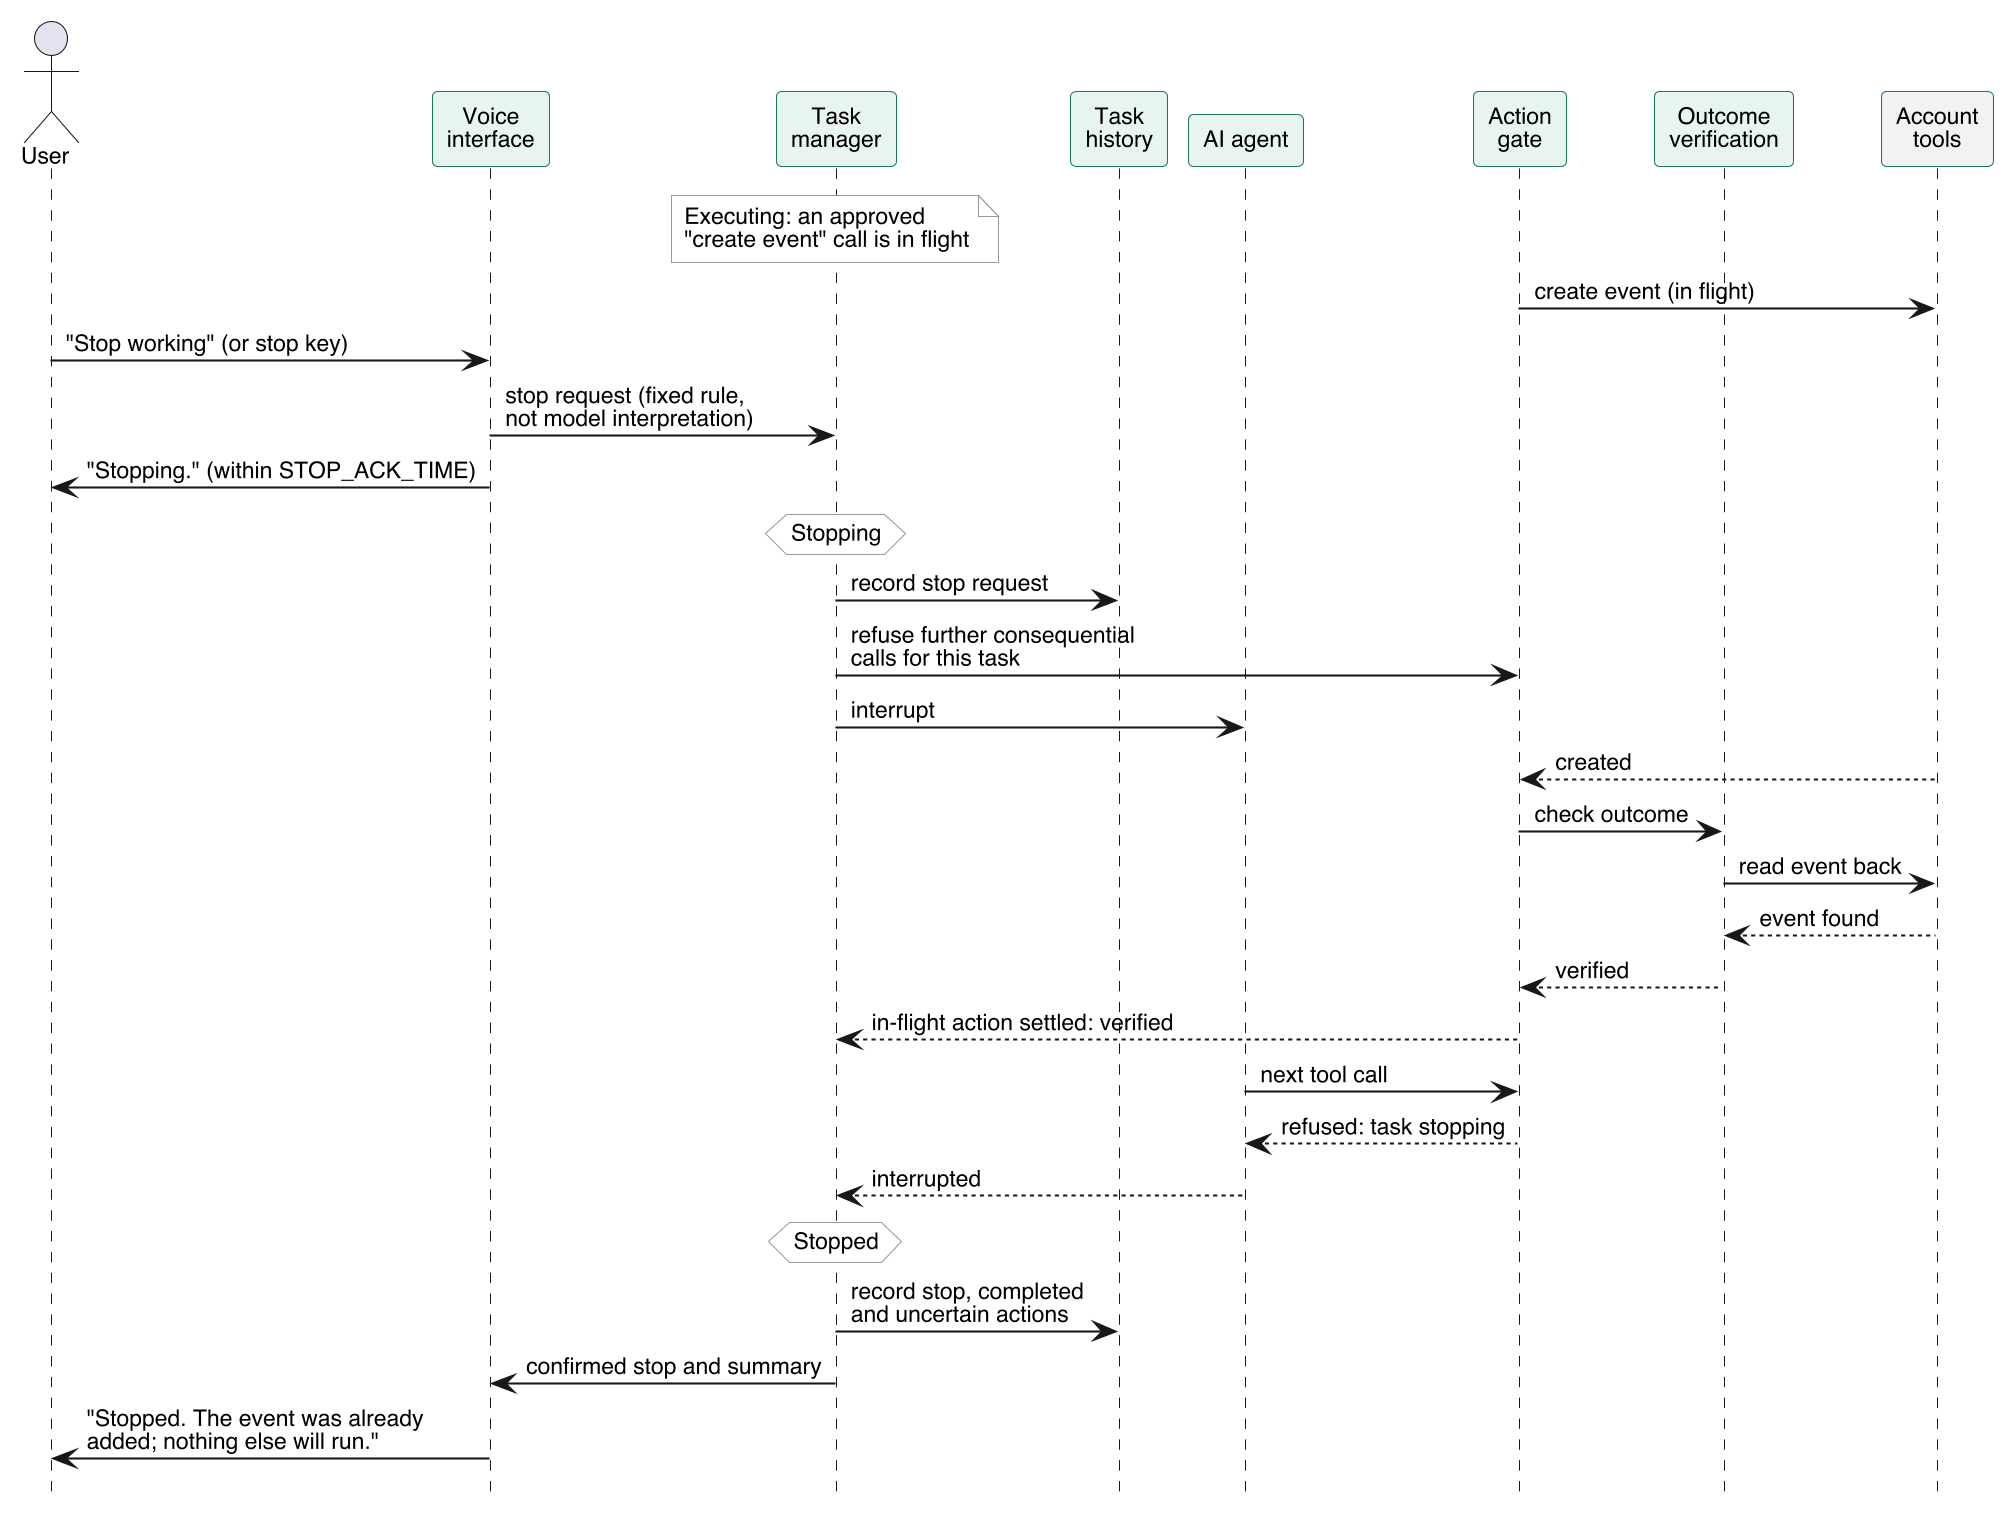
\includegraphics[width=\textwidth,height=.78\textheight,keepaspectratio]{figures/sequence-stop.png}
\caption{Pausing work while an approved action is in flight.}
\label{fig:seqstop}
\end{figure}

\Needspace{8\baselineskip}
\nsection{S.6 Detailed usage scenarios}

The five use cases below expand the high-level scenarios in G.5. Each lists the main success scenario and its extensions. Extensions are numbered by the step they branch from: ``2a'' branches from step 2.

\Needspace{12\baselineskip}
\subsection*{UC1: Reply to an email}
\addcontentsline{toc}{subsection}{UC1: Reply to an email}

\textbf{Primary actor:} User

\textbf{Preconditions:} A session is active, Gmail is connected through the account tools, and no other task is active.

\textbf{Trigger:} ``Reply to Alex Chen's invitation and say Friday at 2 works for me.''

\textbf{Main success scenario:}
\begin{enumerate}
    \item The voice interface passes the request to the task manager. It starts the task.
    \item The agent searches the inbox (read-only) and finds the invitation.
    \item The agent prepares the reply without saving a draft. The gate holds the send and requests approval.
    \item The system reads back the recipient, subject, and full body: ``Send to Alex Chen, subject Re: Invitation: Thanks for the invitation, Friday at 2 works for me. Send it?''
    \item The user says ``Yes, send it.''
    \item The gate sends the reply with a unique action ID. Outcome verification finds the matching message in Sent.
    \item The user hears ``Your reply was sent to Alex Chen.'' The task history records the request, approval, action, and outcome.
\end{enumerate}

\textbf{Extensions:}
\begin{itemize}
    \item \textbf{2a.} Two possible contacts match. The system asks which one (FR4). It waits for the answer and repeats the question on request (FR5).
    \item \textbf{4a.} The body exceeds SHORT\_MESSAGE\_LENGTH. The system reads the recipient and subject. It summarizes the body and offers a full read-back (FR9).
    \item \textbf{4b.} The user says ``change Friday to Monday.'' That detail changes and is read back. Earlier approval no longer applies (FR16, FR9).
    \item \textbf{5a.} The user declines or requests another task. Approval is withdrawn. The user hears that this reply was not sent (FR20).
    \item \textbf{6a.} The send cannot be confirmed. The system reports failure only with evidence of failure. Otherwise it reports unknown (FR12).
\end{itemize}

\textbf{Success guarantee:} Only the approved reply is sent to the intended recipient. The reported result matches the sending evidence. Delivery or reading by the recipient is not claimed.

\textbf{Failure guarantee:} Nothing is sent without approval of its exact recipient and text. The user hears whether sending was confirmed or remains uncertain.

\Needspace{12\baselineskip}
\subsection*{UC2: Add an event from a webpage to the calendar}
\addcontentsline{toc}{subsection}{UC2: Add an event from a webpage to the calendar}

\textbf{Primary actor:} User

\textbf{Preconditions:} A session is active, Google Calendar is connected, and the page is public or has a saved login (FR23).

\textbf{Trigger:} ``Add the meetup on this page to my calendar.''

\textbf{Main success scenario:}
\begin{enumerate}
    \item The task manager starts the task. The user hears a short acknowledgment.
    \item The browser opens the page. A clear non-essential cookie prompt is rejected under FR24.
    \item The agent reads the event title, date, time, and place (read-only).
    \item The agent proposes event creation. The gate holds it. The system reads back the details.
    \item The user approves.
    \item The gate creates the event with a unique action ID. Outcome verification checks the returned details or a matching calendar record.
    \item The user hears the verified result (Figure~\ref{fig:seqnormal}).
\end{enumerate}

\textbf{Extensions:}
\begin{itemize}
    \item \textbf{2a.} The consent prompt is unclear. The system asks the user before choosing an option (FR24).
    \item \textbf{3a.} The page tells the agent to ignore the user or send information elsewhere. The system treats this text as data. It does not follow those instructions (FR13).
    \item \textbf{3b.} The end time is missing. The system asks instead of guessing (FR4).
    \item \textbf{3c.} A matching event already exists. The system reports it before asking for approval.
    \item \textbf{5a.} The user declines. No event is created. The system reports this.
\end{itemize}

\textbf{Success guarantee:} The calendar contains one approved event. A matching creation response or calendar record confirms its details.

\textbf{Failure guarantee:} No event is created without approval. Uncertain creation is reported as unknown.

\Needspace{12\baselineskip}
\subsection*{UC3: Compare information on a website}
\addcontentsline{toc}{subsection}{UC3: Compare information on a website}

\textbf{Primary actor:} User

\textbf{Preconditions:} A session is active. The site is public, or its login was saved through the vault page (FR23).

\textbf{Trigger:} ``On this conference site, compare the standard and student tickets.''

\textbf{Main success scenario:}
\begin{enumerate}
    \item The task manager starts the task.
    \item The agent navigates without making a consequential change. Clear non-essential cookie prompts follow FR24.
    \item The agent gathers each ticket's price and what it includes.
    \item The user hears a short comparison limited to the request. Uncertain details are stated. For example, fees may be unclear (FR18, FR12).
    \item The user corrects the request: ``Only compare tickets that include workshops.''
    \item The agent rechecks and reports the corrected comparison (FR6). Nothing is purchased or submitted.
\end{enumerate}

\textbf{Extensions:}
\begin{itemize}
    \item \textbf{2a.} A saved login exists. The agent uses it only on its intended site (FR23).
    \item \textbf{2b.} No login is saved. The system explains the private setup route. The task pauses for setup.
    \item \textbf{2c.} The site requests a one-time code or push approval. The user may speak the code or approve on their device (FR23).
    \item \textbf{2d.} The site requires a device-bound passkey. The system explains the manual handoff when that requirement becomes known.
    \item \textbf{5a.} The user asks to buy a ticket. This requires approval of the purchase details. It follows the approval and verification flow in UC1.
\end{itemize}

\textbf{Success guarantee:} The comparison matches the site and the corrected request. Unconfirmed details are stated.

\textbf{Failure guarantee:} No purchase or submission bypasses approval. Authentication follows FR23.

\Needspace{12\baselineskip}
\subsection*{UC4: Correct or pause a running task}
\addcontentsline{toc}{subsection}{UC4: Correct or pause a running task}

\textbf{Primary actor:} User

\textbf{Preconditions:} A task is active.

\textbf{Trigger:} The user says ``stop working'' or presses the stop key.

\textbf{Main success scenario:}
\begin{enumerate}
    \item The user requests a pause while an approved event creation is in progress.
    \item The voice interface recognizes the stop phrase and says ``Pausing work'' within STOP\_ACK\_TIME (FR3, NFR3).
    \item The task manager enters Pausing. The gate blocks new task actions. Unused approvals are withdrawn. Safely cancellable work is interrupted.
    \item The submitted event creation cannot be cancelled safely. It returns a matching event record. The system records that result (FR8, FR12).
    \item The task enters Paused. The user hears ``Paused. The event was already added. The remaining work has not run.''
    \item The user may ask questions while work stays paused. A clear request to continue resumes the task after state checks. Any remaining writes need fresh approval.
\end{enumerate}

\textbf{Extensions:}
\begin{itemize}
    \item \textbf{1a.} The user corrects the task instead. The agent receives the correction (FR6). Changed action details require fresh approval (FR9).
    \item \textbf{1b.} The user says only ``stop.'' Speech stops and work pauses. The system asks what the user wants next (FR3).
    \item \textbf{4a.} A form was prepared but not submitted. Its context is saved where possible. The system says it was not submitted. Resumption requires a check that the page still matches the request.
    \item \textbf{4b.} The earlier submission times out. The task remains paused. The system reports its outcome as unknown. Reconciliation may continue without advancing the task. It does not retry blindly (FR11).
    \item \textbf{6a.} The user cancels. The task enters Cancelling and then Cancelled. Earlier actions are reported and are not undone automatically.
\end{itemize}

\textbf{Success guarantee:} No new task action starts after the recognized stop request until the user resumes. Checks may only reconcile earlier actions. The user hears what completed and what remains.

\textbf{Failure guarantee:} An uncertain external result stays labelled unknown. A confirmed pause is not presented as cancellation of an earlier submission.

\Needspace{12\baselineskip}
\subsection*{UC5: Reconnect without duplicating an action}
\addcontentsline{toc}{subsection}{UC5: Reconnect without duplicating an action}

\textbf{Primary actor:} User

\textbf{Preconditions:} A task is active and the connection drops.

\textbf{Trigger:} The connection to the user is lost.

\textbf{Main success scenario:}
\begin{enumerate}
    \item The task pauses (FR7). The client signals connection loss within CONNECTION\_NOTICE\_TIME. A local sound is used if network speech is unavailable (NFR.Sa.2).
    \item The user reconnects, or starts a new session later.
    \item The system briefly reports the task's state: what completed, what was pending, and anything uncertain (FR18, FR21).
    \item The user says ``continue.'' The system checks relevant state before resuming. Any unused approval is requested again.
\end{enumerate}

\textbf{Extensions:}
\begin{itemize}
    \item \textbf{1a.} Approval was pending. It is withdrawn. On reconnection the user hears that the pending action was not executed. Resumption needs fresh approval (FR20).
    \item \textbf{1b.} An action was already submitted. Its outcome is checked before a retry. The same action ID never executes twice (FR11).
    \item \textbf{4a.} The user cancels instead of continuing. The task ends after cancellation handling. The user hears what had already completed.
\end{itemize}

\textbf{Success guarantee:} No completed action is repeated as a retry. The user hears the task state before it continues.

\textbf{Failure guarantee:} Uncertain state is reported. Work does not resume silently.

\Needspace{8\baselineskip}
\nsection{S.7 Prioritization}

\begin{itemize}
    \item Must (POC, by November 23, 2026): FR1 to FR3, FR8, FR9, NFR3.
    \item Must (before participant evaluation): FR4 to FR7, FR10 to FR16, FR18 to FR24, NFR1, NFR5, NFR.E.1 to NFR.E.4.
    \item Should (tune with usability evidence): conversational timing, FR17, NFR2, NFR4.
\end{itemize}

The POC shall demonstrate approval and work-stop controls for its selected email/calendar and browser workflows. This demonstrates feasibility for the tested action paths; it does not establish coverage of every integration or website action.

\Needspace{8\baselineskip}
\nsection{S.8 Verification and acceptance criteria}

\begin{itemize}
    \item Each functional requirement shall have at least one test using synthetic data and test accounts. Detailed procedures belong in the V\&V Plan.
    \item Approval tests shall check writes and consequential commitments. No tested consequential action may start without matching approval. Tests shall also cover autonomous navigation and the FR24 exception.
    \item Pause tests shall cover a lookup and a submitted write. Record acknowledgment time and the time new actions are blocked. Verify that later results are reported accurately. A voice reconnection shall not resume work by itself.
    \item Recovery tests shall cover uncertain outcomes and stale approvals. A completed action shall not be repeated as a retry.
    \item Outcome tests shall use a meaningful connector response, a matching record, and a website confirmation. A queued request shall not be reported as delivered. Insufficient evidence shall produce an unknown result.
    \item Voice tests shall cover pauses within a sentence and short acknowledgments. They shall also cover corrections, interrupted explanations, and status requests. Record premature replies and missed interruptions. Use participant feedback to tune timing.
    \item Privacy checks shall verify that application history and logs exclude authentication codes. Provider processing and retention shall be reviewed separately.
    \item State properties P1 to P6 (S.9) shall be checked against recorded events. NFR2 shall be measured on a declared task suite. Report all attempts and failures.
\end{itemize}

\Needspace{8\baselineskip}
\nsection{S.9 Formalization: task state machine}

Each task has one state $q \in Q$, where
$Q = \{$Working, AwaitingClarification, AwaitingApproval, Executing, Pausing, Paused, Cancelling, Cancelled, Done, Failed$\}$.
The partial transition function $\delta : Q \times \Sigma \to Q$ uses the events in Table~\ref{tab:fsm}. Figure~\ref{fig:states} summarizes task control.

The running states are Working, AwaitingClarification, AwaitingApproval, and Executing. Pausing, Paused, and Cancelling are also active states. Cancelled, Done, and Failed are final. A session has at most one active task.

A work-stop request blocks new task actions as soon as it is recognized. Pausing records this change and requests safe interruption. It then enters Paused. An earlier external operation may still be pending. Its outcome is tracked separately. Reconciliation checks may continue while paused. They may not advance the task. The report distinguishes unfinished work from unknown outcomes.

Cancellation uses Cancelling to block new actions and preserve earlier results. It then enters Cancelled. Earlier operations are not undone. An unresolved external submission does not justify repeating it.

Pending approvals are withdrawn on pause, disconnection, or cancellation. They do not expire merely because a connected user takes time to answer. Resumption requires a clear instruction and a check of relevant state. Unused writes need fresh approval. A new voice session alone does not resume work. New requests follow FR19.

\begingroup
\small
\begin{xltabular}{\textwidth}{>{\raggedright\arraybackslash}p{3.5cm}>{\raggedright\arraybackslash}X>{\raggedright\arraybackslash}p{3.4cm}}
\caption{Task state transitions}\label{tab:fsm}\\
\toprule
\textbf{From} & \textbf{Event} & \textbf{To}\\
\midrule
\endfirsthead
\toprule
\textbf{From} & \textbf{Event} & \textbf{To}\\
\midrule
\endhead
\bottomrule
\endfoot
Working & required details missing or ambiguous & AwaitingClarification\\\addlinespace[4pt]
AwaitingClarification & user answers & Working\\\addlinespace[4pt]
Working & user corrects the task & Working\\\addlinespace[4pt]
Working & consequential action or batch proposed & AwaitingApproval\\\addlinespace[4pt]
AwaitingApproval & explicit approval of exact details & Executing\\\addlinespace[4pt]
AwaitingApproval & user declines or changes details; pending action not run & Working\\\addlinespace[4pt]
Executing & item outcome recorded; approved batch items remain & Executing\\\addlinespace[4pt]
Executing & last approved item outcome recorded & Working\\\addlinespace[4pt]
Working & all requested outcomes confirmed & Done\\\addlinespace[4pt]
Working & no way to continue; remaining outcomes reported & Failed\\\addlinespace[4pt]
any running state & work-stop request or bare ``stop''; dispatch blocked & Pausing\\\addlinespace[4pt]
any running state & disconnect or provider outage; dispatch blocked & Pausing\\\addlinespace[4pt]
Pausing & context saved; safe interruption requested; outstanding operations recorded & Paused\\\addlinespace[4pt]
Paused & status question, reconnection alone, or another stop request & Paused\\\addlinespace[4pt]
Paused & clear resume instruction; relevant state checked; blocking uncertainty resolved & Working\\\addlinespace[4pt]
any running state, Pausing, or Paused & explicit cancellation or confirmed task replacement & Cancelling\\\addlinespace[4pt]
Cancelling & dispatch blocked; context and outstanding operations recorded & Cancelled\\\addlinespace[4pt]
\end{xltabular}
\endgroup



Required properties:
\begin{itemize}
    \item P1: A write or consequential commitment starts only in Executing with matching approval. FR24 is the sole cookie-rejection exception.
    \item P2: Changed details invalidate approval. Pause, disconnection, cancellation, and task replacement withdraw all unused approvals.
    \item P3: A recognized work-stop request blocks new task actions until explicit resumption. Only checks of earlier outcomes may proceed. Pause feedback reports any external work still pending.
    \item P4: Final task states do not resume execution. Later evidence may update an earlier action's outcome in history.
    \item P5: Each consequential action has a recorded approval of its exact details before execution. Each approved batch item has a unique ID and executes at most once. FR24 is the stated exception.
    \item P6: A session has at most one active task. This includes Pausing and Cancelling.
\end{itemize}

\begin{figure}[htbp]
\centering
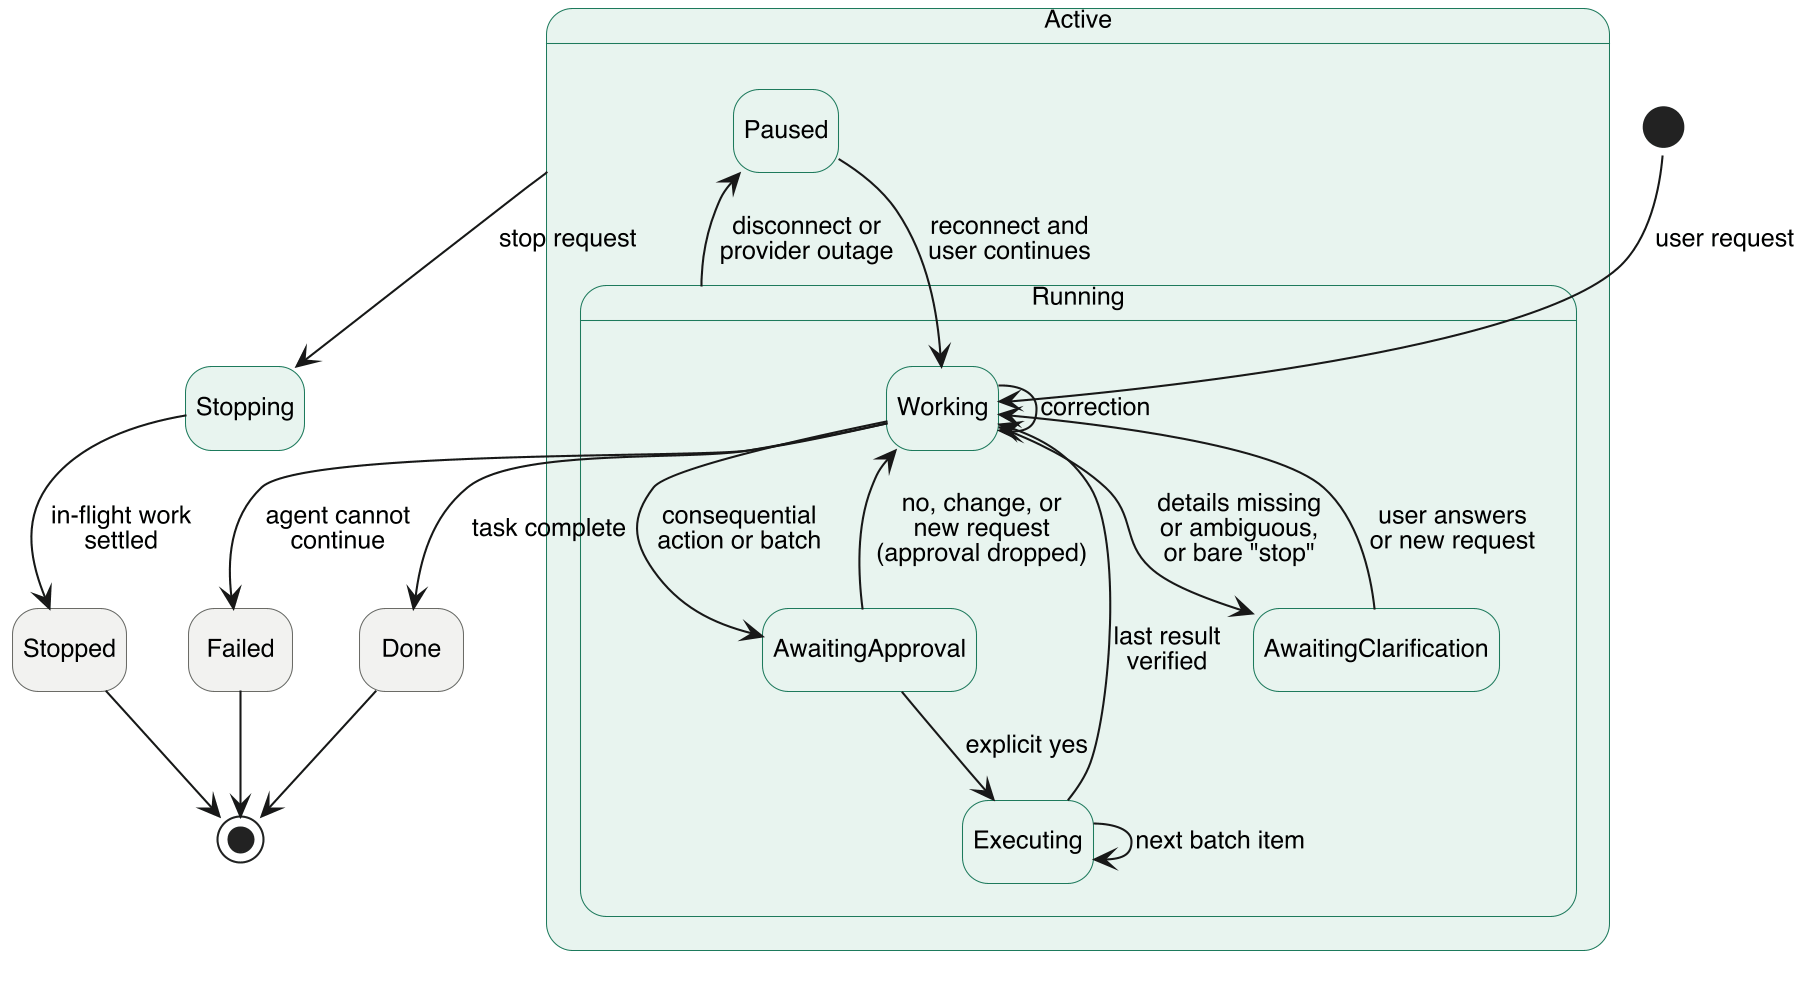
\includegraphics[width=\textwidth,height=.78\textheight,keepaspectratio]{figures/state-diagram.png}
\caption{Task control states. Running groups the four running states in S.9. Grey states are final. External operations are tracked separately.}
\label{fig:states}
\end{figure}

\chapter*{Project}
\addcontentsline{toc}{chapter}{Project book}
\minitoc

\nsection{P.1 Roles and personnel}

As in the Development Plan: voice and client (Lucas, reviewed by Curtis); agent and tools (Aaron, reviewed by Kevin); deployment and reliability (Kevin, reviewed by Aaron); evaluation and quality (Curtis, reviewed by Lucas).

\comment{Decide who writes which SRS sections.}

\nsection{P.2 Imposed technical choices}

\begin{itemize}
    \item Hermes agent harness, LiveKit, Browser Use, Composio (for Gmail and Google Calendar).
    \item Mac, Chrome, English for the initial release.
    \item LaTeX documents in the course template repository; GitHub for issues and reviews.
\end{itemize}

\nsection{P.3 Schedule and milestones}

\begin{itemize}
    \item October 19: SRS and Hazard Analysis.
    \item November 2: V\&V Plan.
    \item November 16: Design document revision minus one; Interview Report.
    \item November 23 to December 3: POC demonstration.
    \item January 18: Design document.
    \item March 8: V\&V Report and Usability Report.
    \item March 31: Final documentation. April 6: EXPO.
\end{itemize}

\nsection{P.4 Tasks and deliverables}

\comment{Break the POC into tasks on the GitHub project board (owner, acceptance criteria, due date) and summarize them here in a table.}

\nsection{P.5 Required technology elements}

\begin{itemize}
    \item LiveKit Agents (Python) and a speech-to-text and text-to-speech provider.
    \item Hermes agent and an AI model provider.
    \item Browser Use with Chromium.
    \item Gmail and Google Calendar APIs through the Composio SDK, our own Google OAuth app before participant sessions, and test accounts.
    \item TypeScript and React for the web client.
\end{itemize}

\nsection{P.6 Risk and mitigation analysis}

\begin{itemize}
    \item Supervision through Hermes may not work as documented: test approvals, interrupts, and reconnection on a pinned version first.
    \item Browser actions may not be interceptable for approval: if not, the browser becomes read-only for the initial release.
    \item Recruitment of blind participants may fail: report technical feasibility only and disclose missing usability evidence.
    \item Provider costs may exceed the budget: meter usage and reconcile monthly.
\end{itemize}

\nsection{P.7 Requirements process and report}

Requirements come from the Problem Statement, Development Plan, Hazard Analysis, TA guidance, prior research, and interviews. An interview with a former DBCS staff member was held on October 17, 2026; FR16 to FR18, the G.8 profile change, and intervenors as stakeholders came from it. Blind participants will be recruited for repeated feedback. Requirements will be revised as POC results and interview findings arrive.

\chapter*{Requirement dependencies}
\addcontentsline{toc}{chapter}{Requirement dependencies}

\comment{Build a traceability matrix: goals G1 to G5 against FR1 to FR24, NFRs, and FR.Sa requirements.}

\chapter*{Likely and unlikely changes}
\addcontentsline{toc}{chapter}{Likely and unlikely changes}

\begin{itemize}
    \item Likely: replacing the AI model, speech provider, or agent harness; adding account services; changing timing constants after measurement.
    \item Unlikely: dropping the approval rule for consequential actions; dropping voice as the main interaction.
\end{itemize}

\chapter*{References}
\addcontentsline{toc}{chapter}{References}

\renewcommand{\bibsection}{}
\bibliographystyle{plainnat}
\bibliography{../../refs/CapstoneSources}

\comment{WCAG, AODA, and the Google API policy are now cited in E.7/E.3. LiveKit, Hermes, Browser Use, WebAIM, and Morae are named in the Glossary, P.2, P.5, and the System book but not yet marked with \textbackslash citep; add those where each is first mentioned. The Meyer handbook is already linked inline on the first page.}

\chapter*{Appendix: AI use disclosure}
\addcontentsline{toc}{chapter}{Appendix: AI use disclosure}

Aaron Loh used Claude Code (Claude Opus 5.5) to work through the requirements. It asked questions, summarized tool documentation, and translated the team's decisions and Kevin's requirements draft into this structured draft. Aaron made and reviewed every decision. The team will review, verify, and rewrite this draft before submission.

OpenAI Codex assisted with the October 17 layout and consistency review. It also helped revise the supervision requirements and simplify the System section from Aaron's decisions. Team review is pending.

\comment{Other members: add the tools you used.}

\chapter*{Appendix: Reflection}
\addcontentsline{toc}{chapter}{Appendix: Reflection}

\comment{Each member answers the SRS reflection questions from their own experience.}

\input{../Reflection.text}

\input{../SRS_Reflection.text}

\end{document}
